% !TEX root = thesis.tex

\subsection{QGP in Small systems}
\label{sec:smallsystem}
After the existence of QGP in heavy-ion collisions has been established, attention has been turned to small systems. Proton-proton (\pp) and proton-Lead (\pPb) collisions have been studied at LHC and RHIC has studied a host of different collision systems; namely proton--gold (p--Au)~\cite{Aidala:2016vgl}, deuteron--gold (d--Au)~\cite{Adler:2003ii,Arsene:2003yk,Back:2003ns,Adams:2003im} and helium$^3$--gold ($^3\mbox{He--Au}$)~\cite{Adare:2015ctn} collisions starting from 2000. %At LHC small systems have been studied in proton-Lead (pPb) collisions. First observations seemed to indicate that the signals taken to confirm the existence of QGP in heavy-ion collisions disappear in these small systems.

Already before the era of modern colliders, collective behaviour in proton-proton collisions was considered by names like Heisenberg, Fermi and Bjorken~\cite{Nagle:2018nvi}. Eventually there were some experimental searches of QGP in \pp and $p\bar p$ collisions in E735 at Tevatron~\cite{Alexopoulos:1993wt} and MiniMAX~\cite{Brooks:1999xy}. However no conclusive evidence was found. 

In the early years of RHIC these small systems were mostly considered as control measurement, for example in constraining nuclear modified parton distribution functions (nPDFs) that determine the initial gluon distributions that determine the first epoch of heavy-ion collisions~\cite{Shen:2015qta, Adare:2015lcd}. 

In 2010 ultrahigh-multiplicity \pp collisions were studied at CMS~\cite{Khachatryan:2010gv}. The study found that particles had a weak but clear preference to be emitted along a common transverse $\phi$ angle across all rapidities ~\cite{Salgado:2016jws}. This seemed like behaviour were similar to AA collisions, but it was argued that it could as well come from momentum correlations present in the earliest moments of the collision.

In 2012 LHC ran its first \pPb data taking period. Around the same time d--Au data was re-examined at RHIC. Now it was revealed that most of the flow signatures attributed to hydrodynamic expansion in AA collisions also existed in smaller systems.



%-Sub nucleonic structure needed to describe intial conditions in pA, \pp
%\FloatBarrier

\subsubsection{Collective phenomena}
The most rugged analysis of collective behaviour concerns the two (or more) particle correlations, often parametrised via the relative azimuthal angle and pseudorapidity differences, $\Delta \phi$ and $\Delta \eta$ respectively. Figure~\ref{fig:smallsystems2} shows two-particle correlations measurements in \PbPb, \pPb and \pp collisions at the LHC~\cite{Aad:2015gqa}. In \PbPb collisions long-range correlations dominate over short-range phenomena. This shows in the two ridges at $\Delta \phi = 0 $ and $\Delta \phi = \pi$. At $\Delta\phi\approx\Delta\eta\approx0$, there is a peak coming from single jet fragmentation. Since the away-side jet can be spread out in $\Delta\eta$, this contribution disappears when compared to the flow contribution at the away side ridge. In \pPb, and \pp the near side peak is more distinguished and the away-side jet contribution starts to show. Still, one can see long-range correlations that seem like flow-like collective behaviour in both systems. 
\begin{figure}[b!]
\centering
            	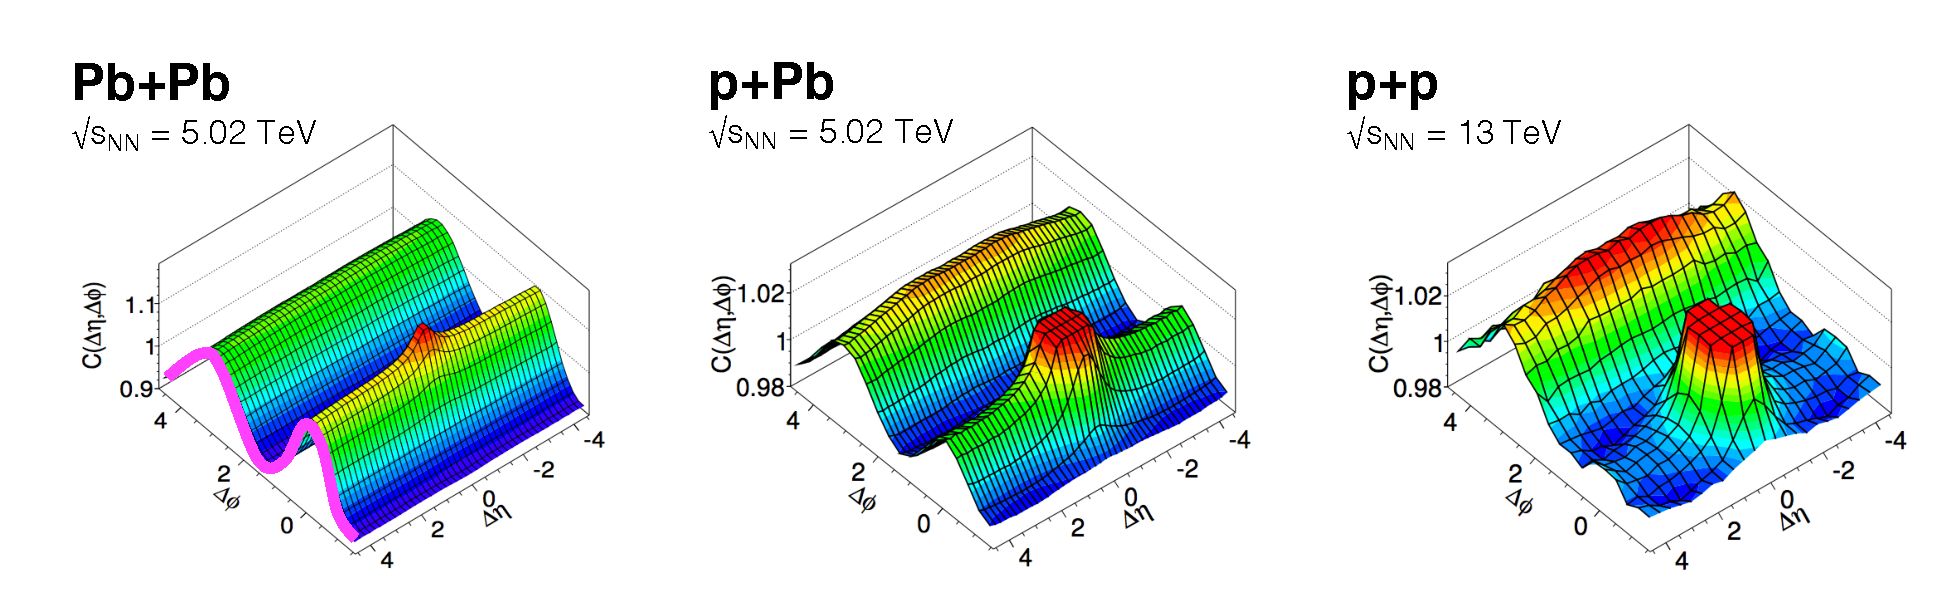
\includegraphics[width=0.9\textwidth]{pics/figure_ridges}
                \caption{Two-particle correlation results in \PbPb, \pPb, and \pp collisions at the LHC~\cite{Aad:2015gqa} }
	\label{fig:smallsystems2}
\end{figure}

In addition to the two particle correlations, correlations have been observed in the form of $v_n$ coefficients both at LHC~\cite{Acharya:2017ino} and at RHIC~\cite{Aidala:2016vgl}. The results have also been described  with hydrodynamical models, although the applicability of said models might be questionable, because of the large Reynolds numbers in small systems~\cite{Shen:2016zpp,Niemi:2014wta}. Figure~\ref{fig:smallsystems1} shows results for $v_2$ in different collisions systems at RHIC as measured by PHENIX and Figure~\ref{fig:smallhydro} shows the eccentricities and the resulting hydrodynamic evolution in the systems. These different systems provide also different initial geometries. d--Au collisions naturally have an ellipsoidal form, while a $^3\mbox{He--Au}$ collision has a triangular form and thus produces larger triangular flow, $v_3$ components. 

\begin{figure}[htb]
\centering

		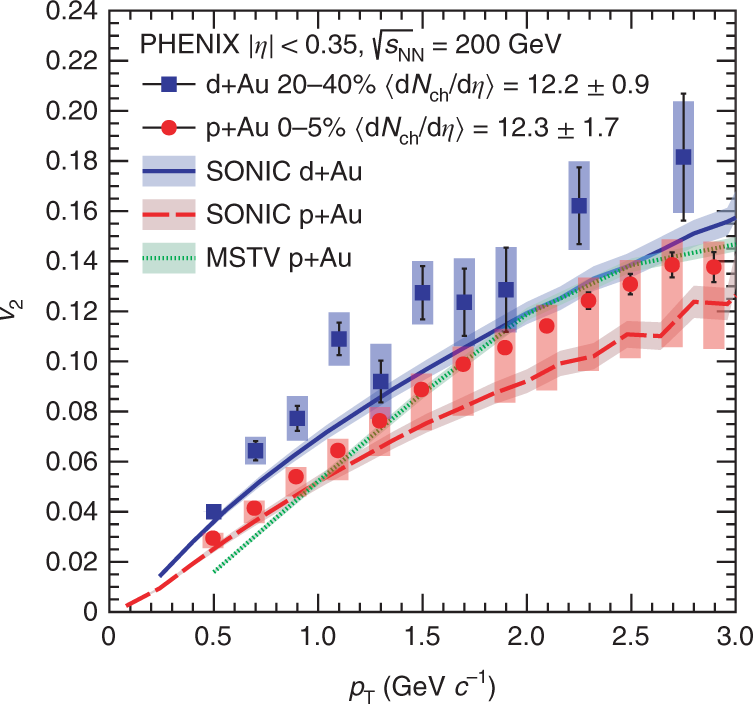
\includegraphics[width=0.5\textwidth]{figures/41567_2018_360_Fig4_HTML.png}
                \caption{Comparison between hydrodynamic calculations and data from $\mbox{p--Au}$, $\mbox{d--Au}$ and $^3\mbox{He--Au}$ collisions~\cite{PHENIX:2018lia}}
	\label{fig:smallsystems1}
\end{figure}

\begin{figure}[b!]
\centering
            	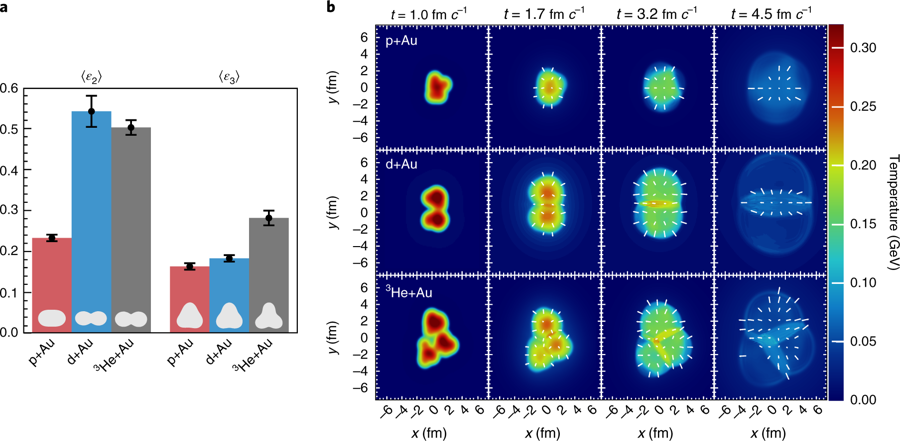
\includegraphics[width=\textwidth]{figures/PhenixNature_1.png}
	\caption{\emph{left:} Eccentricities in different systems. \emph{right:} Calculations of the initial energy density in small collision systems at RHIC and the resulting hydrodynamic evolution~\cite{PHENIX:2018lia}.}
	\label{fig:smallhydro}
	\end{figure}


%Citation to ALICE result for mass ordered v2
Other observations that produce flow-like results include mass ordered $v_2$ coefficients~\cite{CMS:2018rfr} and higher order harmonics coming from fluctuations in the initial geometry~\cite{Acharya:2017ino}. Thus all the major collective flow phenomena observed in heavy-ion collisions have been also identified in small systems.

One open question is identifying the point the point, where flow-like correlations end. The question has proved challenging since low multiplicity events are dominated by non-flow phenomena. This makes observations in low multiplicity events model/method dependant. Different methods assess non-flow contributions differently. Thus some methods fail to observe a signal in cases, where others do and it is unclear whether this is true collective motion or it comes from non-flow contributions.

%\FloatBarrier

\subsubsection{Absence of jet quenching}
In A+A collisions, an important confirmation of the standard model comes from the energy loss of high $\pt{}$ partons traversing the medium, as discussed in Section~\ref{sec:energyloss}.
%referred to as jet quenching~\cite{Gyulassy:2003mc,doi:10.1146,Accardi:2009qv}.
Originally the interest in small systems was due to ruling out possible cold nuclear matter effects that might affect the results also in $\PbPb$. In 2003 the jet quenching effect was observed to disappear in d--Au collisions at RHIC~\cite{Adler:2003ii,Adams:2003im,Arsene:2003yk,Back:2003ns}. This was taken as an indication that no QGP was created. Similarly at LHC no jet modification has been observed in \pPb collisions. Figure~\ref{fig:smallsystems3} shows the nuclear modification factor $R_{\mathrm{pA}}$ and $v_2$ in \pPb collisions as measured at the LHC~\cite{Khachatryan:2016odn,Aad:2014lta}. 

Now the lack of jet modification seems surprising considering the multitude of flow observations supporting the existence of QGP in small systems. One possible explanation is simply the size of medium. In \PbPb collision partons traversing through the medium lose energy to the medium. If the medium is very small there is limited time for interaction with the medium. Reaction plane dependent $R_{AA}$ measurements~\cite{Adler:2006bw} in \PbPb collisions indicated that \unit[2]{fm} could be the minimum path length required for energy loss.

Some calculations~\cite{Zhang:2013oca,Park:2016jap,Tywoniuk:2014hta} indicate that there should be modification in the most central \pPb collisions, but selecting these in the analysis is complicated~\cite{Nagle:2018nvi}. In \PbPb collisions most of the particle production comes from the medium and thus the total multiplicity is a good indicator of centrality. However in \pPb collisions the total multiplicity is smaller and is more strongly influenced by jet phenomena. Events with jets have naturally larger multiplicities and are more likely to be classified as central events.

So far the only observable indicative of jet quenching in \pPb collisions is the high $\pt{}$ $v_2$. In heavy-ion collisions this is not explained by hydrodynamics. Instead it is assumed to come from jet quenching with different path lengths through the medium in different directions. In Figure~\ref{fig:smallsystems3} ATLAS~\cite{Aad:2014lta} and CMS~\cite{Sirunyan:2017pan} measurements of $v_2$ in \pPb and \PbPb collisions are shown. The \pPb results seem to follow a very similar pattern. However, the non-flow effects in this high-\pt{} region are not fully under control, so the physical interpretation is still under debate. 


\begin{figure}[b!]
\centering
            	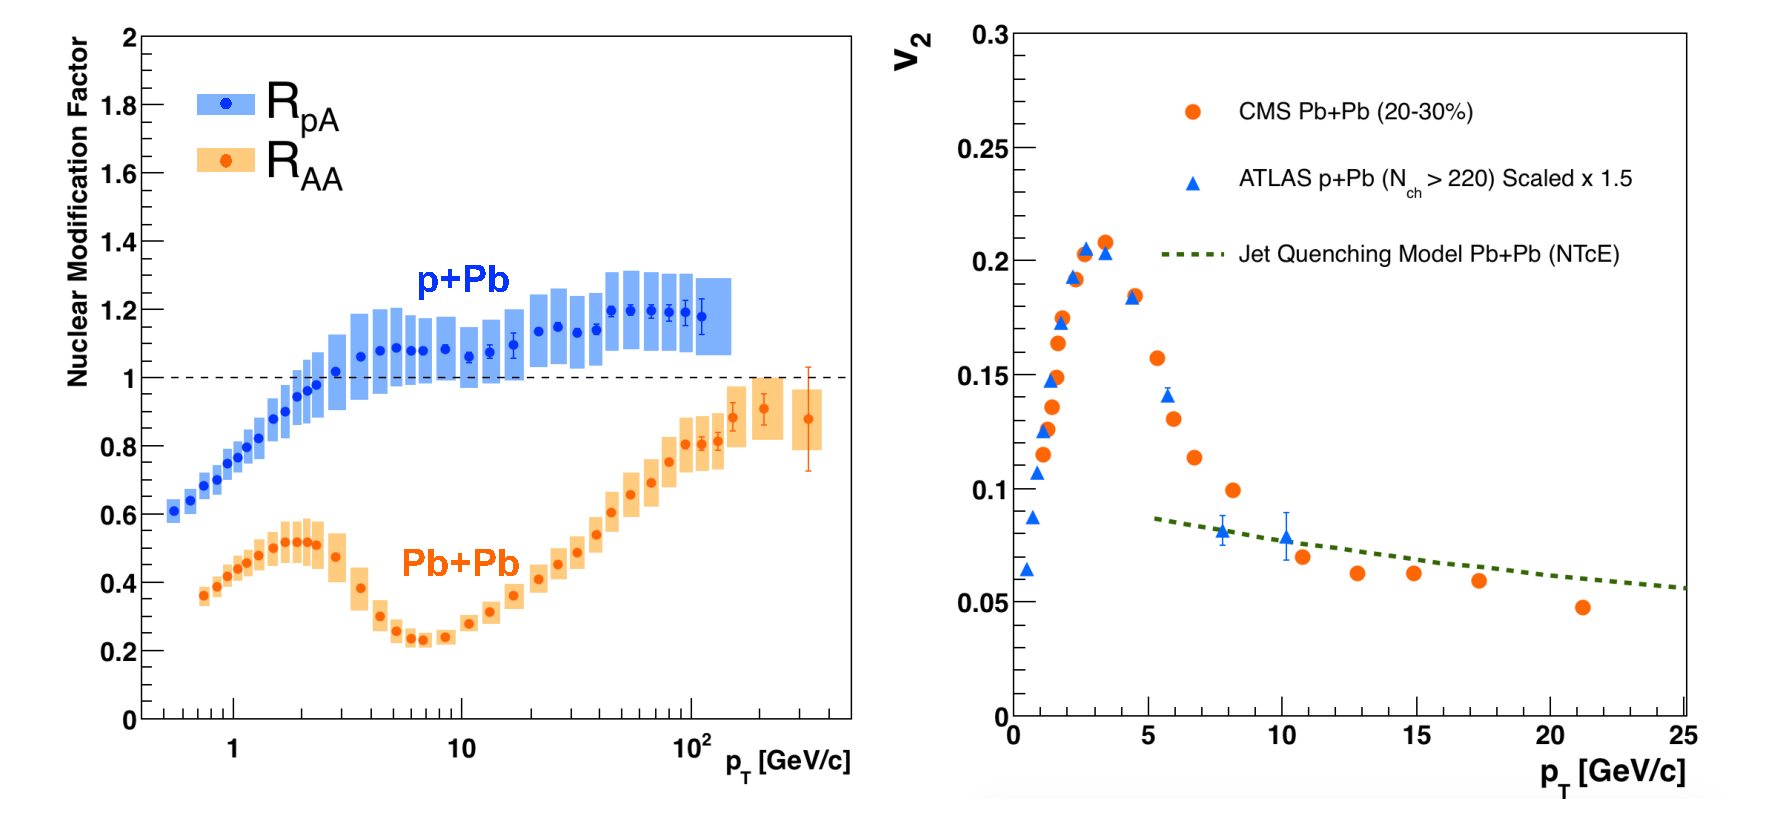
\includegraphics[width=0.9\textwidth]{pics/figure_ppb_jetquenching.pdf}
                \caption{\emph{left:}The nuclear modification factor $R_\mathrm{pA}$ in \pPb collisions~\cite{Khachatryan:2016odn}. Compared to $R_\mathrm{AA}$  $R_\mathrm{pA}$ shows no sign of modification. 
                \emph{right:} The $v_2$ coefficient as a function of \pt{} in \PbPb and \pPb at the LHC~\cite{Aad:2014lta,Sirunyan:2017pan}. For shape comparison the \pPb results have been scaled up by a factor 1.5. The green dotted curve ~\cite{Zhang:2013oca} is from a jet quenching calculation where the anisotropy results from the directional dependence of the
energy loss, rather than hydrodynamic flow.}
                
	\label{fig:smallsystems3}
\end{figure}


%\begin{table}[htb]
%\centering
%\caption{Summary of observations in small system}
%\label{tab:Smallsystem}
%\begin{tabular}{ l | c | c | r }
%  Observable & \PbPb & \pPb & \pp \\
%    \hline			
%  Jet RpA/RAA & Modified & No modification &  - \\
%  Hadron RpA/RAA & Modified & No modification &  -\\
%  Heavy flavors & & & \\
% % Jet quenching & Observed & No  \\
%  Jet shape & Broadening & No observations & - \\
%  Two-particle correlations & Ridge & Ridge & Ridge  \\
%  $v_2$ & Observed & Observed & Observed \\
%  Mass ordered flow & & & \\
%  Higher ordered harmonics & &  &\\
%  High $\pt{}$ $v_2$ & Observed & Maybe & - \\
%  \hline
%  \end{tabular}
%  \end{table}

\FloatBarrier
\subsubsection{Centrality determination in small systems}
\label{sec:smallsystemcentrality}
In lead-lead collisions the total multiplicity of the event is a good indicator of the geometric centrality of the collision~\cite{Abelev:2013qoq}. In proton-lead collisions the connection between multiplicity and centrality is less clear~\cite{Adam:2014qja}. In \pPb collisions the impact parameter is only loosely correlated to $N_\mathrm{part}$ or $N_\mathrm{coll}$. Hence, although one uses traditionally the term centrality to refer to these measurements, the relevant parameters are $N_\mathrm{part}$ and $N_\mathrm{coll}$~\cite{Adam:2014qja}.

\begin{figure}[b!]
\centering
            	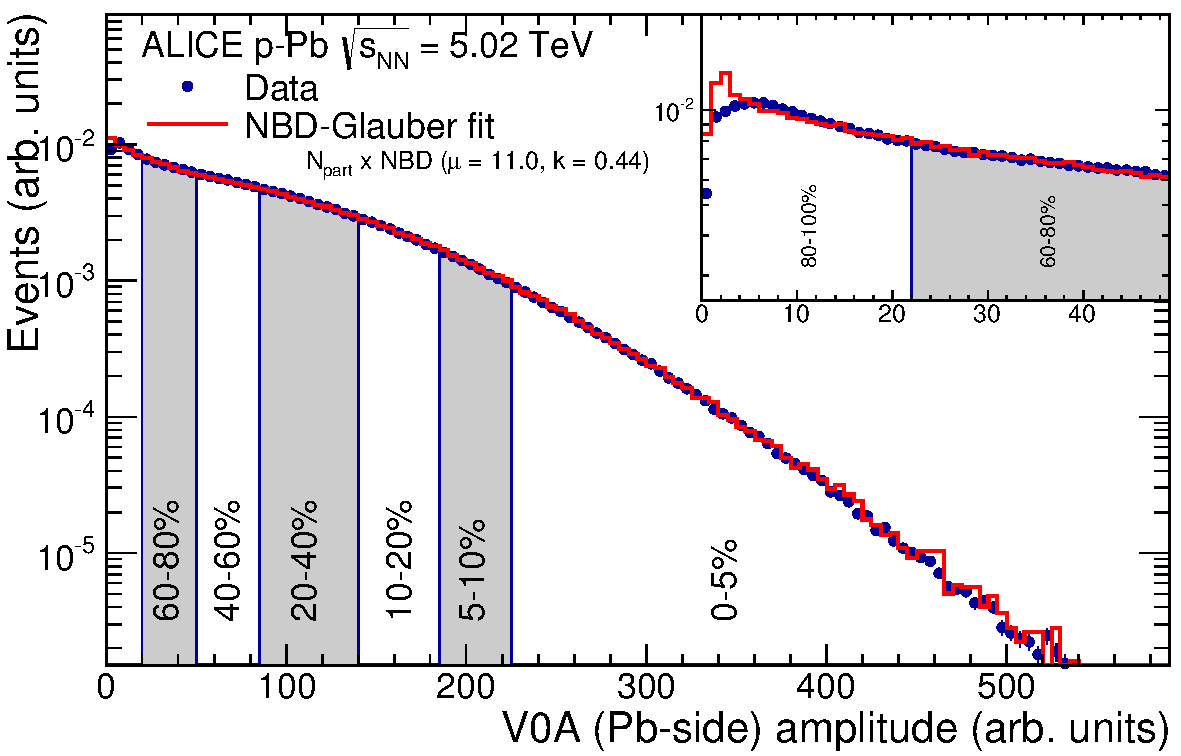
\includegraphics[width=0.750\textwidth]{pics/CentralitypPb}
                \caption{Distribution of the sum of amplitudes in the V0A hodoscopes (Pb-going), as well
as the NBD-Glauber fit. Centrality classes are indicated by vertical lines. The
inset shows a zoom-in on the most peripheral events.~\cite{Adam:2014qja}}
	\label{fig:pPbcentrality}
\end{figure}




As in \PbPb collisions the Glauber model~\cite{Miller:2007ri} is generally used to calculate geometrical quantities of \pPb collisions. In this model, the impact parameter $b$ controls the average number of participating nucleons $N_\mathrm{part}$ and the corresponding number of collisions $N_\mathrm{coll}$. It is expected that variations of the amount of matter overlapping in the collision region will change the number of produced particles, and parameters such as $N_\mathrm{part}$ and $N_\mathrm{coll}$ have traditionally been used to describe those changes quantitatively, and to relate them to \pp collisions. Figure ~\ref{fig:pPbcentrality} shows the measured V0A amplitude distribution in ALICE and the best NBD Glauber fit to the distribution~\cite{Adam:2014qja}.



%In practice centrality is determined in \pPb~collisions using the same methods as in \PbPb~collisions.

The problem in \pPb collisions is that fluctuations in multiplicity coming from for example hard scatterings are of the same order as the differences in multiplicity between centrality classes. In \PbPb collisions these multiplicity fluctuations have little influence on the centrality determination as the range of $N_\mathrm{part}$ or $N_\mathrm{coll}$ is large and both $P\left(M|N_\mathrm{part}\right)$ and $P\left(M|N_\mathrm{coll}\right)$ converge quickly to a Gaussian with a small width relative to the range of $N_\mathrm{part}$/$N_\mathrm{coll}$. This is illustrated in Figure~\ref{fig:pPbMult}. In practice selecting high multiplicity in \pPb one chooses not only large average $N_\mathrm{part}$, but also positive multiplicity fluctuations leading to deviations from the binary scaling of hard processes. These fluctuations are partly related to qualitatively different types of collisions. High multiplicity nucleon-nucleon collisions show a significantly higher mean transverse momentum. They can be understood either as harder collisions with larger momentum transfer $Q^2$ or as nucleon-nucleon collisions where multiple parton-parton interactions (MPI) take place. 

\begin{figure}[tb]
\centering
            	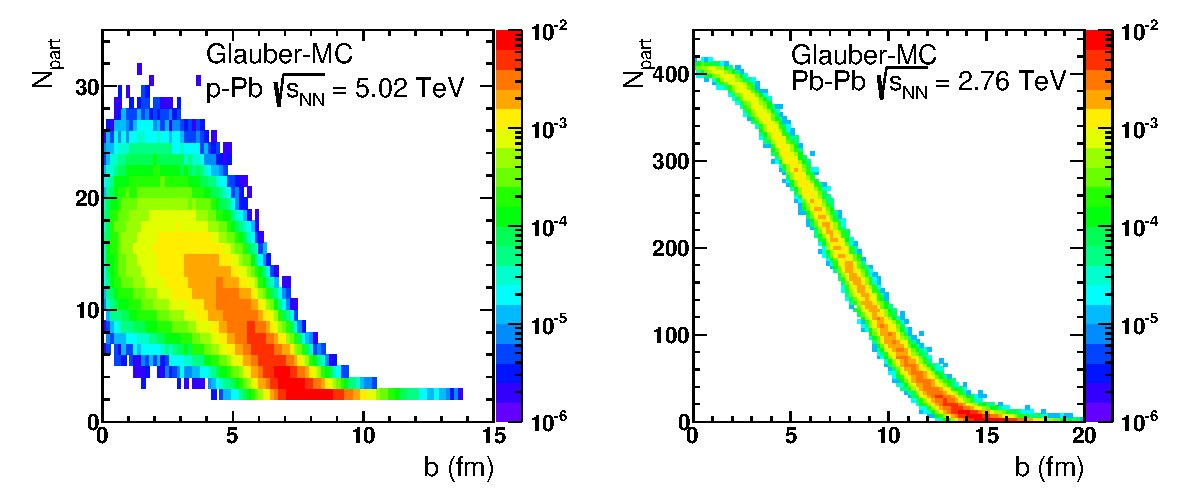
\includegraphics[width=0.7\textwidth]{pics/BNpart_Glau-10758.pdf}
            	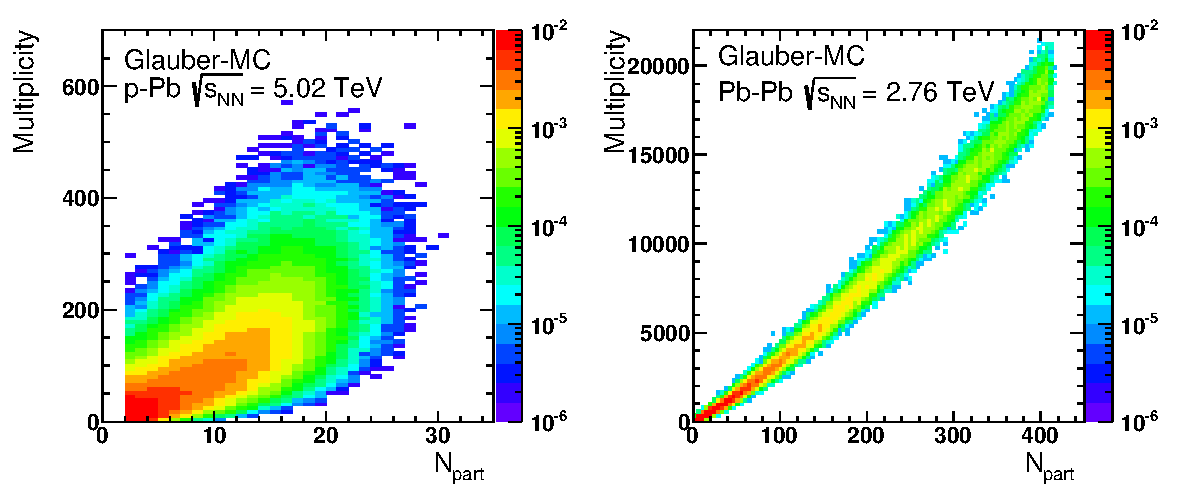
\includegraphics[width=0.7\textwidth]{pics/NpartMult_Glau-10759.pdf}
                \caption{Top: Scatter plot of number of participating nucleons versus impact parameter; Bottom: Scatter plot of multiplicity versus the number of participating nucleons from the Glauber fit for V0A. The quantities are calculated with a Glauber Monte Carlo of p-Pb (left) and Pb-Pb (right) collisions.~\cite{Adam:2014qja}}
	\label{fig:pPbMult}
\end{figure}

Of particular interest are estimators from kinematic regions that are causally disconnected after the collision. The measurement of a finite correlation between them unambiguously establishes their connection to the common collision geometry. Typically these studies are performed with observables from well separated pseudorapidity ($\eta$) intervals, e.g. at zero-degree (spectators, slow-nucleons, deuteron break-up probability) and multiplicity in the rapidity plateau.

One centrality selection that is argued not to induce a bias on the binary scaling of hard processes is provided by the energy measurement with the Zero Degree Calorimeters (ZDC) in ALICE, due to their large $\eta$-separation from the central barrel detectors. They detect the "slow" nucleons produced in the interaction by nuclear de-excitation processes or knocked out by wounded nucleons~\cite{Sikler:2003ef}.





Additional kinematic biases exist for events containing high-$\pt{}$ particles, which arise from the fragmentation of partons produced in parton-parton scattering with large momentum transfer. Their contribution to the overall multiplicity increases with increasing parton energy and thus can introduce a trivial correlation between the centrality estimator and the presence of a high-$\pt{}$ particle in the event. For very peripheral collisions, the multiplicity range that governs the centrality for the bulk of soft collisions can represent an effective veto on hard processes. For the nuclear modification factor this would lead to $R_\mathrm{pPb} < 1$~\cite{Adam:2014qja}.

%{\color{red} More citations to final discussion?}

